\documentclass[11pt]{article}
%DECLARATIONS
\usepackage{graphicx}
\usepackage{xcolor}
\usepackage{placeins}
\usepackage{enumitem}
\usepackage{minted}
\usepackage{hyperref}
%\usepackage[dvipsnames]{xcolor}
\usepackage{fancyvrb}
\usepackage{tcolorbox}
\usepackage{tikz}
\usetikzlibrary{shapes.multipart, calc}
\renewcommand\familydefault{\sfdefault}
\usepackage{tikz-dependency}
\usepackage{moreverb}
\usepackage[linguistics]{forest}
\usepackage{changepage}
\usepackage{float}
\usepackage{caption}
\usepackage{subcaption}
\usepackage{tikz}
\usetikzlibrary{shapes,positioning,calc}
\colorlet{lightgray}{gray!20}

\usepackage[normalem]{ulem}

\depstyle{lvl}{%
    edge height=2.5ex,
    % edge unit distance=#1*2.5ex, % Another way of controlling the appearance of the edges.
    edge below,
    edge horizontal padding=0,
    edge vertical padding=(#1-1)*3ex,
    text only label, % No need for label for functional dependencies.
    edge slant=0, % Right angles
    rounded corners=0,
    edge style={>=triangle 60} % Change the style of the arrowheads.
}
\tikzset{
    matrix/.append style={column sep=0.4cm} % Adding some distance between the attributes.
}
\tikzstyle{TxtBook}=[% Style to mimic the textbook Fundamentals of Database Systems.
    column sep=0cm, % No distance between two attributes.
    nodes={%
        fill=gray!20,
        draw=black,
        inner xsep=3ex,
        inner ysep=1ex
    }
]

\parskip1.5ex
\addtolength{\baselineskip}{+.1\baselineskip}
\newlength{\lineheight}
\setlength{\lineheight}{11pt}
\newcommand{\ls}[1]{\baselineskip=#1\lineheight}
\newcommand{\bitem}{\begin{itemize}}
\newcommand{\eitem}{\end{itemize}}
\newcommand{\benum}{\begin{enumerate}}
\newcommand{\eenum}{\end{enumerate}}
\newcommand{\bdesc}{\begin{description}}
\newcommand{\edesc}{\end{description}}
\newcommand{\comment}[1]{{\color{red}{#1}}}

\usepackage{xcolor}
\usepackage[colorlinks = true,
            linkcolor = blue,
            urlcolor  = blue,
            citecolor = blue,
            anchorcolor = blue]{hyperref}

\newcommand{\MYhref}[3][blue]{\href{#2}{\color{#1}{#3}}}%

% redefine \VerbatimInput
\RecustomVerbatimCommand{\VerbatimInput}{VerbatimInput}%
{fontsize=\scriptsize,
 %
 commandchars=\|\(\), % escape character and argument delimiters for
                      % commands within the verbatim
 commentchar=*        % comment character
}

\newmintedfile[inputsql]{sql}{%
    linenos,
    autogobble,
    breaklines,
}

\newlist{MyIndentedList}{itemize}{4}
\setlist[MyIndentedList,1]{%
    label={},
    noitemsep,
    leftmargin=0pt,
    }
\setlist[MyIndentedList]{%
    label={},
    noitemsep,
    }
    
%BEGIN
\begin{document}
\title{Database Final Project}
\date{\today}
\author{Sahba Tashakkori and Jered Dominguez-Trujillo}

\maketitle
\pagenumbering{gobble}
\begin{center}
\end{center}
\newpage
%\pagestyle{empty}
\tableofcontents
\pagenumbering{arabic}

\pagebreak

\section{Changes Since Proposal}
\noindent
Due to the fact that the 3 data sources, fatality by age, fatality by sex, and fatality by co-morbidity, were gathered only from New York State, not updated frequently, and not comprehensive, we decided to exclude them and instead focus on the remaining 5 data sources from the  \MYhref{https://www.npmjs.com/package/covid19-api}{Covid-19 API}. They are listed below:

\begin{itemize}
    \item \MYhref{https://www.npmjs.com/package/covid19-api}{Covid-19 API}
        \begin{itemize}
        \item \textbf{John Hopkins Data Daily Report}: Data for the 2019 Novel Coronavirus Visual sourced from the Dashboard operated by the Johns Hopkins University Center for Systems Science and Engineering. Updated daily.
        \item \textbf{Tests in US}: Data from 48 states public health labs in the United States, in addition to New York City, USAF, and 9 California counties. Updated daily.
        \item \textbf{USA Medical Aid Distribution}: Tracks medical aid to US hospitals and facilities, including package weight, cost, delivery date of aid to a location and/or hospital. Updated daily.
        \item \textbf{Aggregated Facility Capacity County}: Current population, (occupied) hospital beds, (occupied) ICU beds, healthcare staff, age demographics, grouped by county for the United States. Updated daily 
        \item \textbf{United States Cases By State}: For every state: the number of positive and negative cases, each state's score, number of patients in the ICU and on ventilators, and number of patients who have recovered (supplements the JHU Daily Report with additional fields).
    \end{itemize} 
\end{itemize}

\pagebreak

\section{Introduction}
\label{sec:Intro}
\noindent
Data on global and United States coronavirus (COVID-19) statistics, medical aid, facilities, and demographics will be gathered and organized into a relational database for the eventual purpose of analysis in order to understand the trends and relationships between demographics, testing, geography, hospital systems/availability, medical aid, and political response to the spread and deadliness of the coronavirus. To do this, several sites and APIs that gather and provided updated timeseries data about the coronavirus were studied and evaluated, including \MYhref{https://www.worldometers.info/coronavirus/}{Worldometer}, \MYhref{https://coronavirus.jhu.edu/map.html}{John Hopkins Coronavirus Resource Center}, \MYhref{https://covidtracking.com/api}{The Covid Tracking Project}, and an open source \MYhref{https://www.npmjs.com/package/covid19-api}{Covid-19 API}.

\section{Approach}

\subsection{Sourcing of Data}
\label{subsec:sourcedata}

\noindent
The data sources outlined in \textbf{Section \ref{sec:Intro}} each had unique data: \MYhref{https://www.worldometers.info/coronavirus/}{Worldometer} provides updated positive cases and deaths on a rolling 24-hour basis grouped by country, \MYhref{https://coronavirus.jhu.edu/map.html}{John Hopkins Coronavirus Resource Center} provides geographical data updated frequently, \MYhref{https://covidtracking.com/api}{The Covid Tracking Project} provides data in an easily accessible json format that includes all historical United States positive cases, tests, and deaths data grouped by state, while \MYhref{https://www.npmjs.com/package/covid19-api}{Covid-19 API} provides easily accessibly json data that includes worldwide tests, death, fatality rates, health care system data, and medical aid distribution data that is updated daily and grouped by country, state, city, and county.

\noindent
After analyzing the various data sources available, it was decided that the data will be sourced daily from \MYhref{https://www.npmjs.com/package/covid19-api}{Covid-19 API} since it provides a super-set of the John Hopkins and Worldometer data (which include worldwide current tests, positive cases, and deaths data organized by country) in addition to information on fatality rates, health care systems, and medical aid distribution. This data will all be accessed with normal GET requests using a scripting language such as Python. The data will be accessed daily, after which it will then be parsed and re-organized to a format such a csv file that Oracle Database can easily read, and finally inserted into the final Database to generate a time series of data.

%\noindent
%The data will be sourced from one of the more popular \MYhref{https://covidtracking.com/api}{COVID APIs} \newline (\MYhref{https://covidtracking.com/api}{https://covidtracking.com/api}), which contains cumulative and historical data that will be accessed with normal GET requests using a scripting language such as Python. The data will be retrieved as JSON before being parsed, re-organized, and inserted into the database. 

\pagebreak

\noindent 
Documentation of the various endpoints and data items is included on the \MYhref{https://covid19-docs.chrismichael.now.sh/}{Covid-19 API} website, but we have included a brief outline of the endpoints \textbf{(data items that we are planning to use:}

\begin{itemize}
%    \item \MYhref{https://covidtracking.com/api}{The Covid Tracking Project}
%    \begin{itemize}
%        \item \textbf{States Current Values}: Positive/Negative Tests, Hospitalized, Deaths Organized by State and Periodically Updated Throughout the Day. Contains Data for all 50 States and 6 Territories.
%        \item \textbf{States Historical Data}: Entries from Current Values Saved Everyday and Organized by State at 4 p.m EST. Contains Data for all 50 States and 6 Territories Dating Back to Jan. 22, 2020
%        \item \textbf{US Current Values}: National Cumulative Current Values from States Current Values and Periodically Updated Throughout the Day
%        \item \textbf{US Historical Data}: National Cumulative Historical Values from States Historical Data
%    \end{itemize}
    \item \MYhref{https://www.npmjs.com/package/covid19-api}{Covid-19 API}
        \begin{itemize}
        \item \textbf{John Hopkins Data Daily Report}: Data for the 2019 Novel Coronavirus Visual sourced from the Dashboard operated by the Johns Hopkins University Center for Systems Science and Engineering. Updated daily.
        \item \textbf{Tests in US}: Data from 48 states public health labs in the United States, in addition to New York City, USAF, and 9 California counties. Updated daily.
        %\item \textbf{Fatality Rate By Age}: Global fatality rate grouped by age groups. Updated daily.
        %\item \textbf{Fatality Rate By Sex}: Global fatality rate grouped by sex. Updated daily.
        %\item \textbf{Fatality Rate By Co-morbidity}: Global fatality rate for people with pre-existing conditions. Updated daily.
        \item \textbf{USA Medical Aid Distribution}: Tracks medical aid to US hospitals and facilities, including package weight, cost, delivery date of aid to a location and/or hospital. Updated daily.
        \item \textbf{Aggregated Facility Capacity County}: Current population, (occupied) hospital beds, (occupied) ICU beds, healthcare staff, age demographics, grouped by county for the United States. Updated daily 
        \item \textbf{United States Cases By State}: For every state: the number of positive and negative cases, each state's score, number of patients in the ICU and on ventilators, and number of patients who have recovered (supplements the JHU Daily Report with additional fields).
    \end{itemize} 
\end{itemize}


\noindent
The data will be gathered daily in order to provide historical data to aide in an analysis of trends over time. This will enable the tracking of tests, positive cases, deaths, fatality rate by age, sex, and pre-existing conditions worldwide over time. Additionally, data for the United States regarding medical aid distribution, facility capacity, state cases, ICU occupancy, and ventilator usage will be gathered and stored as a time-series.

%\subsection{Data Items}

%\comment{Might not need this section since the section above explains it}

%\begin{enumerate}
%    \item Number of Positive and Negative Test Results (Per Day and Cumulative)
%    \item Number of Patients who have Recovered (Per Day and Cumulative)
%    \item Number of Patients who have Died (Per Day and Cumulative)
%    \item Number of Patients Hospitalized (Per Day and Cumulative)
%    \item Number of Patients in ICU (\comment{Don't think we have this data})
%\end{enumerate}

%\subsection{Organization of Data}

%\noindent
%My initial thought is to assign a timestamp to each data point that we read. We can probably use a table that has timestamp, newmexico\_id, otherstate\_id
%and then a table that records the statistics for each state (or just incorporate timestamp in the state table). Then we can have some other tables that derive data from the state\_data table or something like that.

\pagebreak

\subsection{Data Analysis}

\noindent
The main function of our work is to create a record of Covid19 related information over time. We will demonstrate the application of the data we gather by performing some sample queries to extract interesting information and trends from the data. We will also use regression to estimate a few trends regarding the disease progression based on the historic data we collected and compare our predictions with the actual data that we ingest in the days after. Some of the trends we may be interested in analyzing include:

\begin{itemize}
    \item Correlation between testing, cases, and number of deaths, and the development over time in different countries/states
    \item Correlation between positive cases, deaths, fatality rates and temperature in each city/state/country over time (i.e. observe how seasonal and geographical temperature changes affect the spread and fatality over time).
    \item Evolution of the fatality rate over time and between demographics.
    \item Correlation between medical aid over time and fatality rate in geographical regions.
    \item Correlation between number of deaths and the number of available hospital beds, ICU beds, and ventilators.
\end{itemize}

\pagebreak

\section{Database Design and Implementation}

\noindent
The database design and implementation for the COVID-19 Timeseries Data is presented as follows:

\begin{enumerate}[1)]
    \item Why a Relational Database (Section \ref{subsec:why})
    \item Approach (Section \ref{subsec:approach})
    \item Database Design (Section \ref{subsec:design})
    \item Database Implementation (Section \ref{subsec:implementation})
    \item Data Insertion and Extraction (Section \ref{subsec:insertextract})
\end{enumerate}

\noindent
It should be noted that the Python file used to collect and prepare the data for database insertion is included as GatherData.py, the SQL files used to create the database and populate the initial STATE table are included as createDB.sql and PopulateStateTable.sql, the SQL file to extract data for analysis using queries is included as Queries.sql, and the Python notebook used to analyze the data and generate the plots seen in Section \ref{sec:analysis} is included as Analysis.ipynb.

\subsection{Why a Relational Database}
\label{subsec:why}
%\noindent
%We will record this data for NM, NY, and the cumulative data from all 50 U.S States. This allows the user of the database to not only compare the trends in NM, NY, but also to examine how the trends in these two states compare to the overall trend in the U.S.


\noindent
The data that we worked with fits into a single machine. Therefore, one of the main motivations behind the NoSQL movement, which was the the ability to distribute relational databases, does not apply to our scenario. In addition, we will not have the "impedance mismatch problem" between our storage and representation formats that NoSQL databases aim to solve \cite{nosqlTalk}. Hence we do not need to use NoSQL solutions, such as document or column based databases, to ease our representation and operations. Moreover, the need for timestamps can be easily solved by adding a timestamp/date column to each entry that keeps track of when the data was recorded and entered. So using a specialized time series database is simply not necessary and results in pointless complications in our approach. We also do not have a data ingestion problem. We will gather the data once per day at a specific time by writing a script to download the data from the website, parses the data, and insert the new data into the database, as described in Section \ref{subsec:insertextract}. For these reasons, a relational database design was chosen to represent the data relationships and to store the COVID-19 data. \\

%\noindent
%Overall, we anticipate that the data gathered can be modeled using a few relations and relationships in the ER model. For example, Medical Aid could be a relation with the relationship 'receives' with the Country/State/City relation. A similar paradigm could be used for a Facilities relation having a relationship with a Country/State/City relation. Additionally, Tests, Positive Cases, and Deaths data could be stored in their own relations, time stamped and given a foreign key that identifies the geographical region it pertains to (Country/State/City). Lastly, given the coarseness of the sampling of the data (daily updates), we do not anticipate that storing time series data in this fashion will pose a problem.

\subsection{Approach}
\label{subsec:approach}

\noindent
Since we worked with 5 different data sources from the \MYhref{https://www.npmjs.com/package/covid19-api}{Covid-19 API}, we approached this problem by first representing each data source as an entity, all related to a parent STATE entity. Since the data provided from the API was largely data from the United States of America, and since the USA has the largest COVID-19 outbreak in the world. it was decided to focus solely on US data and decompose by State. Since the intent was to represent time series data, it was decided that an additional column would be added to each data source that indicated the access/record date. This would allow data to be stored over time in such a way that test data, case data, facility data, and medical aid data could be observed as it changed over time, and the state of the COVID-19 outbreak in the United States on any day could be extracted.


Little approach blurb. Reference Appendix.


\subsection{Database Design}
\label{subsec:design}

\noindent
Little blurb. See next page w\textbf{A note on Normalization}

\FloatBarrier
\begin{figure}[h]
    \centering
    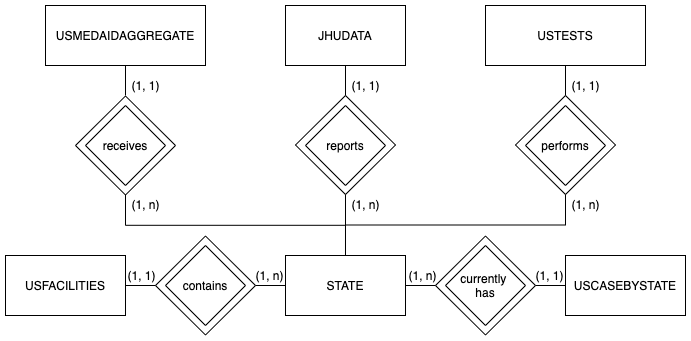
\includegraphics[width=\textwidth]{diagrams/ER2.png}
    \caption{Basic Entity-Relationship Diagram to Model our Data Sources and Relational Database Design}
    \label{fig:er1}
\end{figure}
\FloatBarrier

\FloatBarrier
\begin{figure}[h]
    \centering
    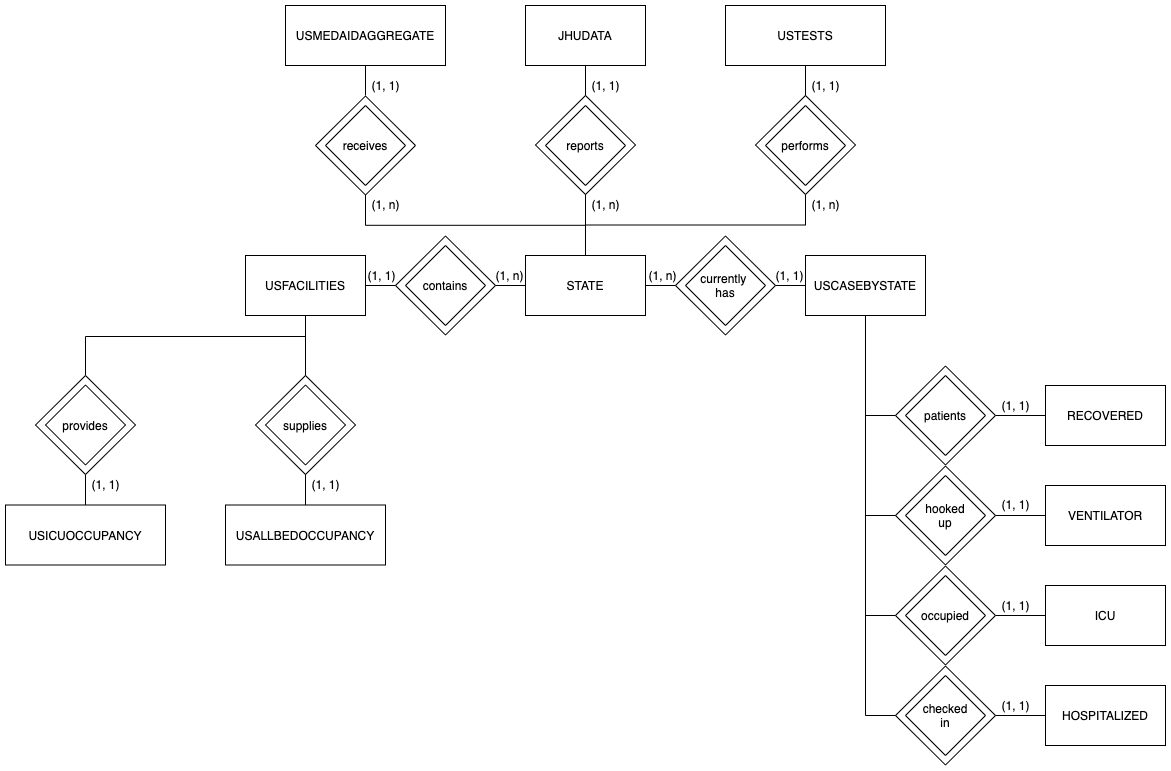
\includegraphics[width=\textwidth]{diagrams/ER1.png}
    \caption{Basic Entity-Relationship Diagram to Model our Data Sources and Relational Database Design}
    \label{fig:er1}
\end{figure}
\FloatBarrier

\subsection{Database Implementation}
\label{subsec:implementation}

\noindent
Little blurb. See next page w\textbf{A note on Normalization}

\pagebreak

\begin{figure}[H]
\begin{adjustwidth*}{}{-4em}
\resizebox{1.5\textwidth}{!}{%
\begin{tikzpicture}[relation/.style={rectangle split, rectangle split parts=#1, rectangle split part align=base, draw, anchor=center, align=center, text height=3mm, text centered}]\hspace*{-0.5cm}

% RELATIONS

\node (statetitle) {\textbf{STATE}};

\node [relation=2, rectangle split horizontal, rectangle split part fill={lightgray!50}, anchor=north west, below=0.6cm of statetitle.west, anchor=west] (state)
{\underline{StateAbbreviation}%
\nodepart{two}   StateName};

\node [below=1.3cm of state.west, anchor=west] (jhutitle) {\textbf{JHUDATA}};

\node [relation=10, rectangle split horizontal, rectangle split part fill={lightgray!50}, below=0.6cm of jhutitle.west, anchor=west] (jhu)
{\underline{DateRecorded}%
\nodepart{two} \underline{Country}
\nodepart{three} \underline{State}
\nodepart{four}  \underline{City}
\nodepart{five}  Confirmed
\nodepart{six} Deaths
\nodepart{seven} Recovered
\nodepart{eight} Active
\nodepart{nine} Latitude
\nodepart{ten} Longitude};

\node [below=1.3cm of jhu.west, anchor=west] (uscasetitle) {\textbf{USCASEBYSTATE}};

\node [relation=8, rectangle split horizontal, rectangle split part fill={lightgray!50}, below=0.6cm of uscasetitle.west, anchor=west] (uscase)
{\underline{DateRecorded}%
\nodepart{two} \underline{State}
\nodepart{three} Positive
\nodepart{four}  Negative
\nodepart{five}  Death
\nodepart{six} Total
\nodepart{seven} DataQualityGrade
\nodepart{eight} DataGrade};

\node [below=1.3cm of uscase.west, anchor=west] (hospitalizedtitle) {\textbf{HOSPITALIZED}};

\node [relation=4, rectangle split horizontal, rectangle split part fill={lightgray!50}, below=0.6cm of hospitalizedtitle.west, anchor=west] (hospitalized)
{\underline{DateRecorded}%
\nodepart{two} \underline{State}
\nodepart{three} HospitalizedCurrently
\nodepart{four}  HospitalizedCumulative};

\node [below=1.3cm of hospitalized.west, anchor=west] (icutitle) {\textbf{ICU}};

\node [relation=4, rectangle split horizontal, rectangle split part fill={lightgray!50}, below=0.6cm of icutitle.west, anchor=west] (icu)
{\underline{DateRecorded}%
\nodepart{two} \underline{State}
\nodepart{three} InICUCurrently
\nodepart{four}  InICUCumulative};
  
\node [below=1.3cm of icu.west, anchor=west] (ventilatortitle) {\textbf{VENTILATOR}};

\node [relation=4, rectangle split horizontal, rectangle split part fill={lightgray!50}, below=0.6cm of ventilatortitle.west, anchor=west] (ventilator)
{\underline{DateRecorded}%
\nodepart{two} \underline{State}
\nodepart{three} OnVentilatorCurrently
\nodepart{four}  OnVentilatorCumulative};
  
\node [below=1.3cm of ventilator.west, anchor=west] (recoveredtitle) {\textbf{RECOVERED}};

\node [relation=3, rectangle split horizontal, rectangle split part fill={lightgray!50}, below=0.6cm of recoveredtitle.west, anchor=west] (recovered)
{\underline{DateRecorded}%
\nodepart{two} \underline{State}
\nodepart{three} Recovered};

\node [below=1.3cm of recovered.west, anchor=west] (facilitytitle) {\textbf{USFACILITIES}};

\node [relation=9, rectangle split horizontal, rectangle split part fill={lightgray!50}, below=0.6cm of facilitytitle.west, anchor=west] (facility)
{\underline{DateRecorded}%
\nodepart{two} \underline{State}
\nodepart{three} \underline{CountyName}
\nodepart{four} Population
\nodepart{five} Population20Plus
\nodepart{six} Population65Plus
\nodepart{seven} StaffedAllBeds
\nodepart{eight} StaffedICUBeds
\nodepart{nine} LicensedAllBeds};

\node [below=1.3cm of facility.west, anchor=west] (allbedtitle) {\textbf{USALLBEDOCCUPANCY}};

\node [relation=4, rectangle split horizontal, rectangle split part fill={lightgray!50}, below=0.6cm of allbedtitle.west, anchor=west] (allbed)
{\underline{DateRecorded}%
\nodepart{two} \underline{State}
\nodepart{three} \underline{CountyName}
\nodepart{four} AllBedOccupancyRate};
  
\node [below=1.3cm of allbed.west, anchor=west] (icubedtitle) {\textbf{USICUBEDOCCUPANCY}};

\node [relation=4, rectangle split horizontal, rectangle split part fill={lightgray!50}, below=0.6cm of icubedtitle.west, anchor=west] (icubed)
{\underline{DateRecorded}%
\nodepart{two} \underline{State}
\nodepart{three} \underline{CountyName}
\nodepart{four} ICUBedOccupancyRate};

\node [below=1.3cm of icubed.west, anchor=west] (medaidtitle) {\textbf{USMEDAIDAGGREGATE}};

\node [relation=5, rectangle split horizontal, rectangle split part fill={lightgray!50}, below=0.6cm of medaidtitle.west, anchor=west] (medaid)
{\underline{DateRecorded}%
\nodepart{two} \underline{State}
\nodepart{three} Deliveries
\nodepart{four} Cost
\nodepart{five} Weight};

\node [below=1.3cm of medaid.west, anchor=west] (testtitle) {\textbf{USTESTS}};

\node [relation=4, rectangle split horizontal, rectangle split part fill={lightgray!50}, below=0.6cm of testtitle.west, anchor=west] (test)
{\underline{DateRecorded}%
\nodepart{two} \underline{DateCollected}
\nodepart{three} CDCLabs
\nodepart{four} USPublicHealthLabs};


  
% FOREIGN KEYS

\draw[-latex] (jhu.three south) -- ++(0,-0.3) -| ($(jhu.one south) + (-2,0)$) |- ($(state.one south) + (0.25,-0.50)$) -| ($(state.one south) + (0.25,0)$);

\draw[-latex] (uscase.two south) -- ++(0,-0.3) -| ($(uscase.one south) + (-2,0)$) |- ($(state.one south) + (0.25,-0.50)$) -| ($(state.one south) + (0.25,0)$);

\draw[-latex] (hospitalized.one south) -- ++(0,-0.3) -| ($(hospitalized.one south) + (-2,0)$) |- ($(uscase.one south) + (0.25,-0.50)$) -| ($(uscase.one south) + (0.25,0)$);

\draw[-latex] (hospitalized.two south) --++(0, -0.3) -| ($(hospitalized.one south) + (-2,0)$) |- ($(uscase.one south) + (0.25,-0.50)$) -| ($(uscase.two south) + (0.25,0)$);

\draw[-latex] (icu.one south) -- ++(0,-0.3) -| ($(icu.one south) + (-2,0)$) |- ($(uscase.one south) + (0.25,-0.50)$) -| ($(uscase.one south) + (0.25,0)$);

\draw[-latex] (icu.two south) --++(0, -0.3) -| ($(icu.one south) + (-2,0)$) |- ($(uscase.one south) + (0.25,-0.50)$) -| ($(uscase.two south) + (0.25,0)$);

\draw[-latex] (ventilator.one south) -- ++(0,-0.3) -| ($(ventilator.one south) + (-2,0)$) |- ($(uscase.one south) + (0.25,-0.50)$) -| ($(uscase.one south) + (0.25,0)$);

\draw[-latex] (ventilator.two south) --++(0, -0.3) -| ($(ventilator.one south) + (-2,0)$) |- ($(uscase.one south) + (0.25,-0.50)$) -| ($(uscase.two south) + (0.25,0)$);

\draw[-latex] (recovered.one south) -- ++(0,-0.3) -| ($(recovered.one south) + (-2,0)$) |- ($(uscase.one south) + (0.25,-0.50)$) -| ($(uscase.one south) + (0.25,0)$);

\draw[-latex] (recovered.two south) --++(0, -0.3) -| ($(recovered.one south) + (-2,0)$) |- ($(uscase.one south) + (0.25,-0.50)$) -| ($(uscase.two south) + (0.25,0)$);

\draw[-latex] (facility.two south) -- ++(0,-0.3) -| ($(facility.one south) + (-3,0)$) |- ($(state.one south) + (0.25,-0.50)$) -| ($(state.one south) + (0.25,0)$);

\draw[-latex] (allbed.one south) -- ++(0,-0.3) -| ($(allbed.one south) + (-2,0)$) |- ($(facility.one south) + (0.25,-0.50)$) -| ($(facility.one south) + (0.25,0)$);

\draw[-latex] (allbed.two south) --++(0, -0.3) -| ($(allbed.one south) + (-2,0)$) |- ($(facility.one south) + (0.25,-0.50)$) -| ($(facility.two south) + (0.25,0)$);

\draw[-latex] (allbed.three south) --++(0, -0.3) -| ($(allbed.one south) + (-2,0)$) |- ($(facility.one south) + (0.25,-0.50)$) -| ($(facility.three south) + (0.25,0)$);

\draw[-latex] (icubed.one south) -- ++(0,-0.3) -| ($(icubed.one south) + (-2,0)$) |- ($(facility.one south) + (0.25,-0.50)$) -| ($(facility.one south) + (0.25,0)$);

\draw[-latex] (icubed.two south) --++(0, -0.3) -| ($(icubed.one south) + (-2,0)$) |- ($(facility.one south) + (0.25,-0.50)$) -| ($(facility.two south) + (0.25,0)$);

\draw[-latex] (icubed.three south) --++(0, -0.3) -| ($(icubed.one south) + (-2,0)$) |- ($(facility.one south) + (0.25,-0.50)$) -| ($(facility.three south) + (0.25,0)$);

\draw[-latex] (medaid.two south) -- ++(0,-0.3) -| ($(medaid.one south) + (-3,0)$) |- ($(state.one south) + (0.25,-0.50)$) -| ($(state.one south) + (0.25,0)$);

\end{tikzpicture}
}%
\end{adjustwidth*}
\caption{COVID-19 Schema}
\end{figure}	

\subsection{Data Insertion and Extraction for Analysis}
\label{subsec:insertextract}

\noindent
The data was collected between 5 MST and 7MST everyday from May 6, 2020 until May 13, 2020 using the \MYhref{https://www.npmjs.com/package/covid19-api}{Covid-19 API} and a python script (GatherData.py). This process involved posting a GET request to the 5 endpoints described in Section \ref{subsec:sourcedata} and obtaining the data in JSON format. 

\noindent
Since some of the data included irrelevant and extraneous columns, the python script first removed those extra columns and converted the data to CSV format to begin prepping for upload to our database instance on Oracle Cloud. Next, since the data needed to be broken down into a file for each of the 11 tables (excluding that STATE table), the python script organized the data into 11 files, taking care that the columns of each CSV file corresponded with the columns of each table in the instance of the database.

\noindent
This allowed the users to run the python script once every evening to collect and organize data, and subsequently upload the data into the Oracle Cloud Database instance. Backups of the raw data obtained from the COVID-19 API endpoints, in addition to backups of the processed data. This process and the results of the analyses from the data entered and extracted from the database is covered in Section \ref{sec:analysis}.

\FloatBarrier
\begin{figure}[h]
    \centering
    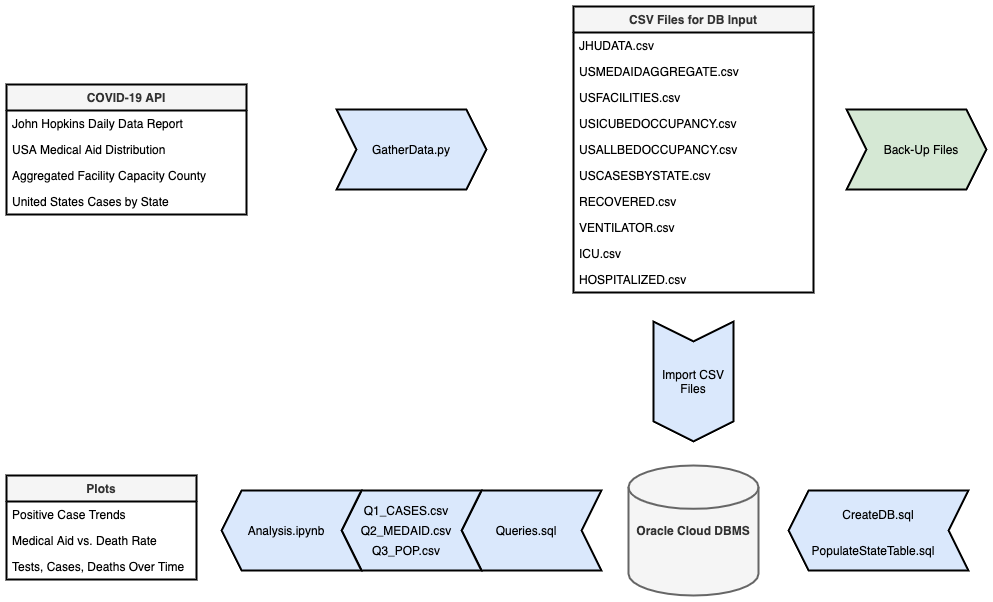
\includegraphics[width=\textwidth]{diagrams/DataInsertionExtraction.png}
    \caption{Data Insertion and Extraction Workflow Overview}
    \label{fig:my_label}
\end{figure}
\FloatBarrier

\pagebreak

\section{Data Analysis}
\label{sec:analysis}

\noindent
We performed a number of analyses to demonstrate the viability of our design and collected data for the kind of analyses that both experts and enthusiasts might be interested in performing. We mainly used SQL queries and Python's data science toolset (Pandas\cite{citepandas}, NumPy\cite{citenumpy}, ScikitLearn\cite{cite_scikit-learn}) to retrieve, prepare, and analyze our data. The following sections provides details on our approach in preparing the data and performing the analysis.

\subsection{Data Preparation}

\noindent
We decided to divide the large tuples of raw data retrieved from our sources into multiple tables as shown in Figure \ref{fig:tbl_bd}. In addition to resulting in a much more logical representation, this approach resulted in far fewer null values in the table. The Python script to retrieve and divide the data resides in the `GatherData.py' file.

\FloatBarrier
\begin{figure}[h]
    \centering
    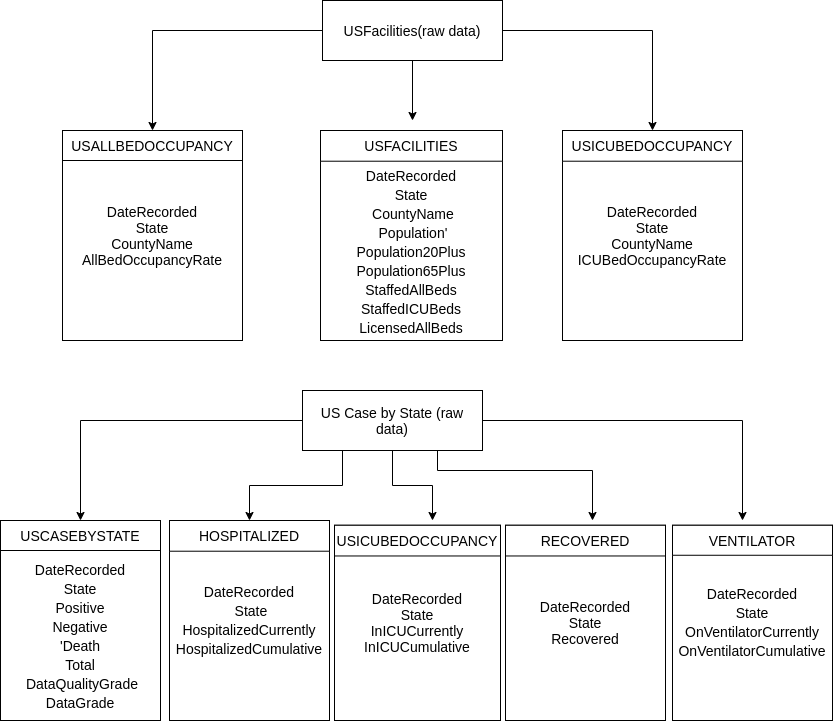
\includegraphics[width=\textwidth]{diagrams/data_breakdown.png}
    \caption{Breaking down the raw data into multiple tables. Note that the arrows simply represent the flow of data and do not connote any database design related concept}
    \label{fig:tbl_bd}
\end{figure}
\FloatBarrier

\noindent
We explored the following items in the data:
\begin{itemize}
    \item Trends in tests, positive and negative cases, and deaths at the State Level
    \item Correlation of tests with medical aid at the state level
    \item Hospital resources as a predictor of death rate
\end{itemize}
In order to perform these analyses, we used simple SQL queries against our database to retrieve the data and simple python scripts to analyze the data and visualize the results. The queries used to retrieve the historic data from our database can be found in the `Queries' folder and the Python scripts for analyzing and visualizing the data can be found in the `analysis.ipynb' Jupyter Notebook.

\subsection{Tests, Cases, and Deaths as the State Level}

\noindent
We started by looking at some of the trends in the data. Figure \ref{fig:pos_trends} shows the number of positive cases in four states for four days (May 6th-9th) and the predictions for two days into the feature using regression.
\subsubsection{Approach}
We used the `USTESTBYSTATES' table to retrieve historical trends for the states. The result of the query was exported to a \textit{csv} file and imported into the python script for plotting and regression analysis.

\FloatBarrier
\begin{figure}[h]
     \centering
     \begin{subfigure}[b]{0.49\textwidth}
         \centering
         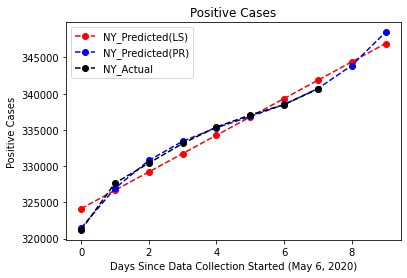
\includegraphics[width=\textwidth]{diagrams/analysis/positive_trend_NY.png}
         \caption{Positive cases trends for NY}
     \end{subfigure}
     \begin{subfigure}[b]{0.49\textwidth}
         \centering
         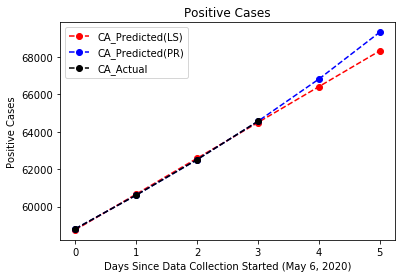
\includegraphics[width=\textwidth]{diagrams/analysis/positive_trend_CA.png}
         \caption{Positive cases trends for CA}
     \end{subfigure}
        \label{fig:three graphs}
             \begin{subfigure}[b]{0.49\textwidth}
         \centering
         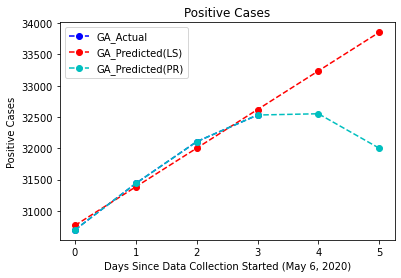
\includegraphics[width=\textwidth]{diagrams/analysis/positive_trend_GA.png}
         \caption{Positive cases trends for GA}
     \end{subfigure}
     \begin{subfigure}[b]{0.49\textwidth}
         \centering
         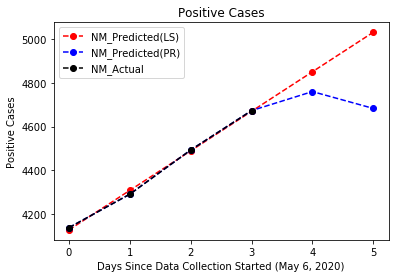
\includegraphics[width=\textwidth]{diagrams/analysis/positive_trend_NM.png}
         \caption{Positive cases trends for NM}
         \label{fig:three sin x}
     \end{subfigure}
        \caption{The actual number of positive cases for CA, GA, NY, NM plus predictions for two days into the future using linear(LS) and plynomal regression (PR3)}
        \label{fig:pos_trends}

\end{figure}
\FloatBarrier

\pagebreak

\subsection{Correlation of Tests with Medical Aid at the State Level}
\noindent
We looked the historical test and medical aid data in our database to look for the relationship between the amount of medical aid a state receives and the number of tests the state performs. 

\subsubsection{Approach}
We joined two tables `USCASEBYSTATE' and `USMEDAIDAGGREGATE', on the timestamp and state attributes and returned the total monetary value of the aid received and the number of tests performed. 

\FloatBarrier
\begin{figure}[h]
    \centering
    
\includegraphics[scale=0.5]{diagrams/analysis/medaid_corr_no_outliers.png}
    \caption{Number of tests conducted vs the amount of medical aid received by states with a line fit through the data using least squares}
    \label{fig:test_cost_fit}
\end{figure}
\FloatBarrier

\FloatBarrier
\begin{figure}[h]
    \centering
    
\includegraphics[scale=0.5]{diagrams/analysis/medaid_corr_outliers.png}
    \caption{Number of tests conducted vs the amount of medical aid received by states with a line fit through the data using least squares}
    \label{fig:test_cost_fit}
\end{figure}
\FloatBarrier


\subsubsection{Discussion}

\pagebreak

\subsection{Hospital Resources as a Predictor of Cases and Deaths}

\noindent
In order to demonstrate a more complex query, we decided to look at the occupancy rate of ICUs and the number of deaths per capita.
\begin{figure}[h]
    \centering
    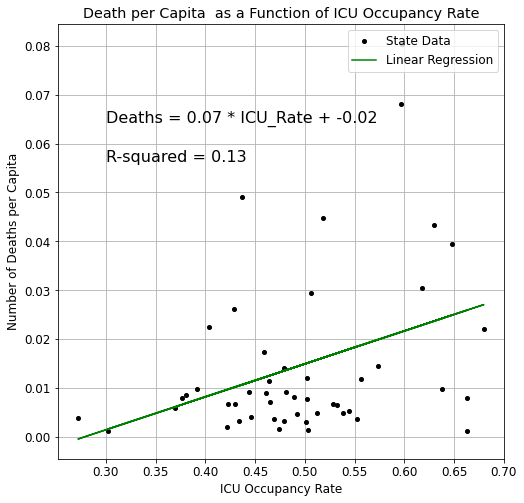
\includegraphics[width=\textwidth]{diagrams/analysis/death_icu.png}
    \caption{Caption}
    \label{fig:my_label}
\end{figure}

\subsubsection{Approach}


\subsubsection{Discussion}

\pagebreak

\section{Conclusions}
..We demonstrated that our design is flexible enough to ingest data from heterogeneous sources and allow for statistical studies on historical Covid19 data...
\section{Future Work}
\bibliographystyle{acm}
\bibliography{refs.bib}

%\appendix

%\section{Original Data From EndPoints}

%\noindent
%JHU CSV Columns :
%\comment{filter on country==us; keep villages, state is foreign key to other tables}:

%\begin{itemize}
%    \item Active
%    \item Combined\_Key
%    \item Confirmed
%    \item Country\_Region
%    \item Deaths
%    \item Last\_Update
%    \item Lat
%    \item Long\_
%    \item Province\_State
%    \item Recovered
%\end{itemize}

%\noindent
%Tests in US CSV Columns (1 Entry for every day since January 18, 2020):
%\comment{own table}:

%\begin{itemize}
%    \item CDC Labs
%    \item DateCollected
%    \item USPublicHealthLabs
%\end{itemize}

%\noindent
%USCasesByState CSV Columns:

%\begin{itemize}
%    \item checkTimeEt
%    \item commercialScore
%    \item dataGrade
%    \item dataQualityGrade
%    \item dateChecked
%    \item dataModified
%    \item death
%    \item fips
%    \item hospitalized
%    \item hospitalizedCumulative
%    \item hospitalizedCurrently
%    \item inIcuCumulative
%    \item inIcuCurrently
%    \item lastUpdateEt
%    \item negative
%    \item negativeRegularScore
%    \item negavtiveScore
%    \item onVentilatorCumulative
%    \item onVentilatorCurrently
%    \item pending
%    \item positive
%    \item positiveScore
%    \item posNeg
%    \item recovered
%    \item score
%    \item state
%    \item total
%    \item totalTestResults
%\end{itemize}


%\noindent
%(Not doing this one) FatalityAge CSV Columns:

%\begin{itemize}
%    \item 3 (Number of Deaths)
%    \item 4 (Without Underlying Conditions)
%    \item 5 (Unknown if with Underlying Conditions)
%    \item 6 (Share of Deaths of Unknown + w/o Conditions)
%    \item Age
%    \item DeathRateAllCases (Share of Deaths)
%    \item DeathRateConfirmed (Number of Deaths)
%\end{itemize}

%\noindent
%(Not doing this one) FatalitySex CSV Columns:

%\begin{itemize}
%    \item 3 (With Underlying Conditions)
%    \item 4 (Share within this Category)
%    \item 5 (Without Underlying Conditions)
%    \item 6 (Share within this Category)
%    \item 7 (Unknown if with Condition)
%    \item 8 (Share within this Category)
%    \item DeathRateAllCases (Share of Deaths)
%    \item DeathRateconfirmed (Deaths)
%    \item Sex
%\end{itemize}

%\noindent
%(Not doing this one) FatalityComorbidity CSV Columns:

%\begin{itemize}
%    \item DeathRateAllCases
%    \item DeathRateConfirmedCases
%    \item Pre-ExistingCondition (Age)
%\end{itemize}

%\noindent
%USMedAid CSV Columns:

%\begin{itemize}
%    \item City
%    \item Cost
%    \item Country
%    \item County
%    \item facility\_type
%    \item first\_shipment
%    \item last\_shipment
%    \item number\_of\_deliveries
%   \item recipient\_Name
%    \item state
%    \item weight\_lbs
%\end{itemize}

%\noindent
%FacilityCapacity CSV Columns:

%\begin{itemize}
%    \item AllBedOccupancyRate
%    \item CountyName
%    \item fips\_code
%    \item ICUBedOccupancyRate
%    \item LicensedAllBeds
%    \item LicensedAllBedsPero1000Adults20\_Plus
%    \item LicensedAllBedsPer1000Elderly65\_Plus
%    \item LicensedAllBedsPer1000People
%    \item Population
%    \item Population\_20\_Plus
%    \item Population\_65\_Plus
%    \item StaffedAllBeds
%    \item StaffedAllBedsPer1000Adults20\_Plus
%    \item StaffedAllBedsPer1000Elderly65\_Plus
%    \item StaffedAllBedsPer1000People
%    \item StaffedICUBeds
%    \item StaffedICUBedsPer1000Adults20\_Plus
%    \item StaffedICUBedsPer1000Elderly65\_PLus
%    \item StaffedICUBedsPer1000People
%    \item State
%\end{itemize}


%\section{Brainstorm}
%\begin{itemize}
%    \item Track fatality, new cases, ... once we have for 3,4 days, we can try to do some sort of regression (jhu, 
%    \item correlation between tests/medical aid (we know what tables we use)
%    \item deaths vs available hospital resources (we use the fragmented tables based on us facilities, 
%    I would get Deaths by State from USCASEBYSTATE
%    I would get hospital resources from USALLBEDOCCUPANCY which is a child table of USFACILITIES
%\end{itemize}




\end{document}
